\documentclass[11pt,fleqn]{article}

\usepackage{vmargin}
\setpapersize{A4}
\setmarginsrb{2.5cm}{2.5cm}{2.5cm}{2.5cm}%
{\baselineskip}{2\baselineskip}{baselineskip}{2\baselineskip}
\setlength{\parindent}{0pt}
\setlength{\parskip}{5pt}

\usepackage{caption}
\usepackage{subcaption}


\usepackage{epsfig}
\usepackage{latexsym}
\usepackage{url}
\usepackage{tgheros}
\renewcommand*\familydefault{\sfdefault}

\newcommand{\eline}{\vspace*{.75\baselineskip}}
\newcommand{\Referee}[1]{\eline \noindent {\bf Reviewer comment #1:} \\}
\newcommand{\Us}{\eline \noindent {\bf Response:}\\}
\newcommand{\TBD}{{\bf To Be Done}}
\newcommand{\newreviewer}[1]{\section*{Reviewer #1}\vspace*{-1.05\baselineskip}}

%\usepackage{tikz}
\usepackage[skins,breakable]{tcolorbox}
\tcbset{textmarker/.style={
%
skin=enhancedmiddle jigsaw,breakable,parbox=false,before skip=-1mm, after skip=0mm,
boxrule=0mm,leftrule=2mm,rightrule=2mm,boxsep=0mm,arc=0mm,outer arc=0mm,
left=2mm,right=2mm,top=2mm,bottom=2mm,toptitle=1mm,bottomtitle=1mm,oversize}}

\newtcolorbox{rcomment}{textmarker,colback=gray!15!white,colframe=gray!80!white}

\newenvironment{revcomment}[1][]
{\Referee{#1}\begin{rcomment}}
{\end{rcomment}}

\usepackage{todo}
\usepackage{hyperref}

%customized
\usepackage{xfrac}
\usepackage{framed}
\newcommand{\highlight}[1]{\begin{framed}%
  \noindent\emph{#1}
\end{framed}}

\expandafter\def\expandafter\quote\expandafter{\quote\itshape}

\graphicspath{{../../}}

\usepackage{xspace}
\newcommand{\ING}{ING\xspace}

% more lenient line breaking (avoids text protruding into margins)
\sloppy

\title{\vspace*{-2cm}{\bf Authors' Response to the Review of
 EMSE-D-24-00354:\\
 ``Understanding Feedback Mechanisms in Machine Learning Jupyter Notebooks''}}

\author{Arumoy Shome, Lu\'{i}s Cruz, Diomidis Spinellis, Arie van Deursen}
\date{}

\begin{document}

\maketitle

\newreviewer{Editor}

\begin{revcomment}

  Despite the paper has significant strengths, there are numerous significant weaknesses that go beyond the process and period of a major revision. Specifically, there are serious concerns about the sampling procedure and the missing details about the inter-rater reliability analysis and recommendations to practitioners.

  Since this paper interests EMSE, I suggest the authors revise and resubmit it as new. When submitting as new, if the authors ask to be assigned to the same editor, I will do my best to assign it to the same reviewers to speed up the revision process.

\end{revcomment}

\Us We thank the editor and reviewers for their valuable feedback, it helped us improve the paper in this new submission. In this document, we address all concerns raised by the reviewers. We have added our response to each comment and added relevant text from the updated manuscript where necessary.

As part of the supplemental material for this submission, we have also included a document which contains the difference between the previous and current submission to make it easier to identify relevant parts of the manuscript that were updated in the new submission.

Please note that despite our best efforts, the excerpts from the manuscript that are included in this document may be outdated. This is because both this document and the manuscript are extensive, and it was challenging to keep everything in sync. Our sincere apologies for this inconvenience. We recommend that when in doubt, the reviewers consult the diff document for the most up-to-date changes that were made in the new submission.

\newreviewer{1}

\begin{revcomment}[1.1]
  The paper presents an insightful exploration of feedback mechanisms within the machine learning (ML) development lifecycle, focusing specifically on Jupyter notebooks authored in Python. By conducting an analysis of ~297.8 thousand notebooks, the authors identify three key feedback mechanisms: assertions as a form of explicit feedback; print statements and last cell statements as forms of implicit feedback. The findings underscore a widespread reliance on implicit feedback mechanisms in Jupyter notebooks. Despite their utility for automated validation, assertions are found to be underutilized, highlighting a significant gap in current testing practices.

\end{revcomment}

\Us Thank you for your valuable comments.

\begin{revcomment}[1.2]
  To date, Jupyter notebooks are pervasively used in the ML development lifecycle, especially in the data preparation and model training phases. Moreover, this year, Python overtook JavaScript as the most popular programming language on GitHub, underscoring a surge in open-source data science and ML projects on the platform [1]. Hence, investigating how data scientists leverage Python Jupyter notebooks in their daily work is a timely and relevant research endeavor, which could inform the evolution of Jupyter Notebook implementations. Also, understanding the nature of feedback mechanisms used in notebooks paves the way to improve overall testing and QA practices in data science projects. In addition, as the authors suggest, this understanding can be useful for optimizing the transition from notebook-based prototyping to production-grade ML code [2].

  The dataset contributed by this study—comprising assertions, print statements, and last-cell statements from notebooks—further enhances its relevance and utility, offering a rich resource for future research.

  Concerning the final discussion, I wonder whether - based on their findings - the authors have thought of any recommendations for designers of notebook platforms (e.g., Jupyter Notebook, Jupyter Lab, Google Colaboratory, etc.). Integrating such recommendations could potentially enhance the practical relevance of this study.
\end{revcomment}

\Us Thank you for your feedback. We have revised section 5.1 Documentation and Technical Debt to incorporate recommendation for notebook users and developers. Here is an excerpt from the manuscript that was added to address this comment.

\begin{quote}
  We recommend that ML practitioners document insights derived from implicit feedback mechanisms, especially for visualizations. Visual cues and trends in visualizations are open to interpretation, meaning that different practitioners may interpret the same plot differently (Heer et al., 2010). By documenting these visual insights, practitioners can ensure that the knowledge encapsulated in the visualizations, along with its interpretation and the subsequent decisions made, is preserved and consistently applied throughout the ML lifecycle. Writing documentation from implicit feedback mechanisms and keeping the documentation up-to-date requires significant manual effort. Therein also lies an opportunity for notebook designers and developers to incorporate automated techniques for generating such documentation. We hope that the dataset contributed by this study provides a valuable resource to develop and evaluate such automated tools.
\end{quote}

\begin{revcomment}[1.3]

  To the best of my knowledge, this study is original and it is the first to explore feedback mechanisms in ML Python Jupyter notebooks. Moreover, the work is well-situated within the existing literature, offering a thoughtful background and context for its findings.

\end{revcomment}

\Us Thank you for your valuable comments.

\begin{revcomment}[1.4]
  The methodology employed in this study generally appears robust and well-structured.

  To address RQ1, the authors undertake an archival study drawing on two distinct sources: GitHub and Kaggle. The unit of analysis, selection criteria for notebooks, and data collection processes are all clearly delineated. However, I suggest that the authors provide additional context about the source platforms for the benefit of researchers who may not be familiar with them - especially Kaggle. Indeed, GitHub and Kaggle have different purposes and present significantly different environments for notebook authoring and sharing.
\end{revcomment}

\Us Thank you for your feedback. We revised Section 3.1 Data Collection to include more information regarding the distinction between Kaggle and Github. Following is an excerpt from the manuscript that was added to address this comment.

\begin{quote}
  Figure 2 illustrates the data collection process employed in this study to gather Jupyter notebooks written in Python from GitHub and Kaggle. GitHub is a popular platform to host and collaborate on software projects. It offers extensive tools for project management such as issue tracking, pull requests, code reviews and tooling for continuous integration and delivery. In contrast, Kaggle is focused specifically on data science and machine learning. It provides integrated computational resources, a rich repository of datasets, and a platform to host machine learning competitions. While GitHub supports formal project workflows, Kaggle encourages a more informal approach to data exploration and modeling, making it a preferred choice for data science practitioners looking for hands-on experience with developing machine learning models.
\end{quote}

\begin{revcomment}[1.5]
  To answer RQ2 and RQ3, the authors delve in a manual analysis of a sample of notebooks, allocating a budget of 200 hours to this task. However, I have the following concerns regarding this procedure.

  \begin{itemize}
    \item The manual task constitutes qualitative coding/annotation, which is inherently subjective. Nonetheless, only a single annotator (the first author) has been involved unless they were ``unable to determine the purpose of the candidate,'' in which case it would be ``additionally analyzed by the second and third author.'' However, for tasks of this type, it is usually advised to involve multiple annotators - at least to code a first, pilot subset of examples, thereby validating the annotation strategy through inter-rater reliability metrics. I recommend that the authors elaborate more on how they addressed potential subjective bias within this annotation process.
  \end{itemize}
\end{revcomment}

\Us Thank you for your valuable feedback. We made several adjustments to the manuscript to address this comment. First, we revised the title of section 3.2 Case Studies to \emph{Exploratory Case Study Analysis} to be more explicit about the scientific methodology used for RQ2 and RQ3. Furthermore, we revised this section to clarify our sampling technique, the potential bias it introduces and how we mitigate this threat. Finally, to mitigate subjective bias of the first author during the first round of annotations, the second author independently conducted a second round of annotations. We have updated the text to describe this process and reported the \emph{Cohen's Kappa} metric for inter-rater agreement.

Following is the entire text from section 3.2 Exploratory Case Study Analysis. We have included the entire section here since we made several revisions to this part of the manuscript.

\begin{quote}
  For RQ2 and RQ3, we allocated a fixed time resource of 200 hours to conduct the exploratory case study analysis of all candidate assertions, print statements and last cell statements. We specified Jupyter notebooks written in the Python programming language as the \emph{site} for the study. To surface interesting candidates for the study, we apply text processing and sampling techniques as described below.

  The assertions, print statements and last cell statements are first tokenized---special characters and alphanumeric words shorter than two characters are removed. Two stop words namely ``assert'' and ``print'' are removed since they appear in all assertions and print statements respectively. The term frequency (TF) for the remaining tokens is calculated and then normalized using their inter-document frequency (IDF). This normalization process assigns higher values to tokens that are less frequently encountered, which can lead to overemphasis of candidates that contain rare tokens. Consider for instance, the trivial print statement \texttt{print("hello, world!")}. Since this statement does not commonly appear in the context of machine learning Jupyter notebooks, it will have a high TF-IDF score but adds little substantive value to the analysis.

  To address the potential bias introduced by this method, we employ stratified random sampling to select candidates for the case study analysis. The subgroups are created based on the aggregated TF-IDF values of the tokens in each candidate. The candidates are then divided into quartiles based on the aggregate value. As a result, all candidates characterized by rare tokens are grouped within a single bin. By randomly selecting candidates from each bin, we ensure that the final population reflects a diverse mix of candidates, mitigating the risk of overrepresenting those that are trivial yet rare.

  During each case study, the first author categorized each candidate using \emph{inductive coding}. The first author analyzed the Python code of the candidate to understand its purpose. Additionally, the entire code cell, the previous cell, next cell and the notebook's purpose was analyzed to bring in rich context. For case studies where the first author was unable to determine the purpose of the candidate, it was additionally analyzed by the second and third authors. Finally, the entire research team held regular meetings throughout this iterative process to ensure consistency in the categorization of the feedback mechanisms.

  A taxonomy of feedback mechanisms observed in ML Jupyter notebooks was created using the categories generated during the exploratory case study analysis. To validate the taxonomy developed by the first author, the second author independently annotated the candidates using the categories developed by the first author. The inter-rater agreement was calculated using the \emph{Cohen's Kappa} method and a score 0.8 was obtained which is regarded as highly agreeable.
\end{quote}

\begin{revcomment}[1.6]

  While it's reasonable to set a predefined time budget for qualitative analysis, and the sampling strategy used seems sound, the number of analyzed notebooks appears quite limited. Consequently, several findings are drawn from an exceedingly small number of ``case studies'', sometimes as few as one. Although the exploratory nature of this study is acknowledged, deriving generalizable conclusions from such isolated instances is challenging. Therefore, it would be advisable for the authors to underscore this limitation more prominently in the Threats to Validity section, and reconsider presenting cases based solely on a single example as definitive findings.
\end{revcomment}

\Us Thank you for your feedback. We made several adjustments to the manuscript to address this comment. First, the title for section 3.2 Case Studies was revised to \emph{Exploratory Case Studies} to emphasize the exploratory nature of this study. Second, we replaced the word ``Finding'' with ``Observation'' in all summary boxes to remind the reader that the results presented in this study are not meant to be generalizable to a population since we conducted qualitative research.

Please note that the diff document does not highlight the changes made to the summary boxes. We tried several different latex implementations to generate the summary boxes but were unable to get it to show in the diff document. Our sincere apologies for this inconvenience.

Finally, we revised the section 4 Results and section 6 Threats to Validity (External Validity) to remind the reader about the qualitative nature of this study.

Following is the text that was added to section 4 Results.

\begin{quote}
  Due to the exploratory nature of this study and the limited number of case studies analyzed, the observations presented should be interpreted with caution and viewed as illustrative rather than definitive. The case studies serve to illustrate key themes, and no definitive conclusions should be drawn from individual instances.
\end{quote}

Following is the text that was added to section 6 Threats to Validity (External Validity).

\begin{quote}
  Furthermore, we would like to reiterate that the case studies presented in RQ2 and RQ3 serve to illustrate key themes, and no definitive conclusions should be drawn from individual instances.
\end{quote}

\begin{revcomment}[1.7]
  Overall, the paper is well-written and well-organized. The explanations provided are clear. The images and charts are well-crafted, providing valuable visual support to the text and enhancing comprehension.

  However, the methodology section lacks specific details about the processes and steps involved in addressing RQ1.
\end{revcomment}

\Us Thank you for your feedback. We revised section 3.1 Data Collection to include more details regarding the steps involved in addressing RQ1. Specifically, we have separated the section into two subsections. Section 3.1.1 Collection of ML Jupyter Notebooks contains text from the last version of the manuscript and describes the data collection procedure to collect the Jupyter notebooks relevant to this study. We added section 3.1.2 Collection of Feedback Mechanisms to the manuscript which describes the steps involved in extracting the feedback mechanisms from the notebooks in further detail.

Following is the text that was added to section 3.1.2 Collection of Feedback Mechanisms.

\begin{quote}
  For RQ1, we extracted the contents of all code cells from the Jupyter notebooks by parsing the underlying JSON structure. We then used the \texttt{ast} module provided by the Python programming language to extract the assert, print and last statements from all code cells.

  The raw contents of each cell were then converted into an AST. The \texttt{NodeVisitor} class from the \texttt{ast} module was used to traverse the AST and collect all \texttt{Assert} nodes. To collect assertions written using Python modules not included in the standard distribution, we also collected all function \texttt{Call} nodes that contain the string ``assert'' in their name. Similarly, all print statements were collected by traversing the AST to find all function \texttt{Call} nodes with the name ``print''. To collect the last statements, we first removed all cells that did not produce any output and consequently extracted the last top-level node from the AST of the code cell. The raw Python code was regenerated from the ASTs using the \texttt{unparse} method provided by the \texttt{ast} module.

  Prior to conducting the analysis for RQ2 and RQ3, we removed duplicate data points resulting in a data set of 27.1 thousand assertions, 498.3 thousand print statements and 373.6 thousand last cell statements.
\end{quote}

\begin{revcomment}[1.8]
  Moreover, the authors have summarized each finding using a summary box; while this is potentially useful to improve the paper understandability, the number of these boxes is high and, in a few cases, the summarized text is shorter than the summary itself (see Sect. 4.3.3) or takes up a comparable space (see Sect 4.3.5). The result is a certain degree of repetition, while it remains challenging to keep the big picture.
\end{revcomment}

\Us Thank you for your feedback. We tried our best to reduce the size of the summary boxes, especially where the boxes are the same size or larger than the main text itself. Almost all summary boxes were revised. Please note however that the diff document does not highlight the changes made to the summary boxes. We tried several latex implementations to generate the summary boxes but were unable to get it to show in the diff document. Our sincere apologies for this inconvenience.

\begin{revcomment}[1.9]
  On a minor note, from Fig. 2 it is not clear how many notebooks were left after applying the filtering criteria.
\end{revcomment}

\Us Thank you for your feedback. We updated section 3.1.1 Collection of Jupyter Notebooks to explicitly mention the number of notebooks that were excluded after applying the filters and the number of notebooks in the final dataset.

Following is an excerpt from the revised text of section 3.1.1 Collection of Jupyter Notebooks relevant to this comment.

\begin{quote}
  Since the focus of this study is on the analysis of Python code, [\ldots] 107 thousand notebooks were excluded after applying the above filters, leaving a dataset of 190.8 thousand notebooks.
\end{quote}

\begin{revcomment}[1.10]

  The methodology adopted in this study is thoroughly described. Moreover, the authors have released the dataset and replication package of this paper on Figshare, under a CC-BY license. Overall, I believe the study should be quite easy to replicate.

  An additional appendix has been shared by the authors, containing the most representative examples referenced in the article. However, this appendix is hosted online on a personal website, rather than being incorporated directly at the end of the paper or included with the replication package. Given that references to this appendix are distributed throughout the paper and considering that publications are ideally self-contained, incorporating the appendix within the paper itself would be preferable. If the appendix is too extensive to be included in full, I recommend publishing it as part of the replication package on Figshare, where its long-term accessibility and persistency can be ensured.
\end{revcomment}

\Us Thank you for your feedback. We have added the appendix to the replication package as a PDF document.

\begin{revcomment}[1.11]

  \textbf{Minor issues}
  \begin{enumerate}
    \item page 4, lines 44-46: ``Jupyter notebooks […] leverage the IPython kernel to execute Python code and extends its capabilities […]'' => ``extend''
    \item page 5, Fig. 1: ``Content of the cell are in the source key'' => ``The content of the cell is in the source key'' as well as ``The raw content of outputs that produce text are under the text key.'' => ``… is …''
    \item page 10, lines 31-33: ``Methods such as […] were frequently used to accomodate for the stochastic nature of ML algorithms and comparing high-dimensional data structures.'' => ``for comparing'' or ``to compare''
    \item page 13, lines 33-34: ``Figure 16 show'' => ``Figure 16 shows''
    \item page 26, lines 35-36: ``Catching data errors are critical'' => ``Catching data errors is critical''
    \item Section 5.3: in addition to the course by Kästner and Kang, other courses covering MLOps and Software Engineering for ML are currently fostering ML testing literacy among data science students. Examples are the course on "Software Engineering for AI-enables Systems" [2, 3] held at the University of Bari (Italy) and at the Universitat Politècnica de Catalunya (Spain), as well as the course "Machine Learning Systems Design" held at ULiege (Belgium) [4].
  \end{enumerate}
\end{revcomment}

\Us Thank you for identifying the minor issues. We have addressed them in the new version of the manuscript.

\newreviewer{2}
\begin{revcomment}[2.1]
  The paper presents an extensive analysis of feedback mechanisms in Jupyter notebooks used for machine learning workflows. By mining a significant dataset of 297.8 thousand notebooks and examining 2.3 million code cells, the authors address a critical area of research that has not received sufficient attention. The paper is well-structured, with clear research questions and a logical progression from dataset construction to findings and recommendations. It offers important insights into the role of feedback mechanisms. However, while the foundation of the work is strong, there are areas where methodological and analytical improvements could further enhance the depth and applicability of the findings.
\end{revcomment}

\Us Thank you for your valuable comments.

\begin{revcomment}[2.2]
  \textbf{Strengths of the Paper}
  \begin{enumerate}
    \item Novelty of the topic: the paper tackles an important issue in machine learning development. By focusing on Jupyter notebooks, a widely used tool in the ML community, the study addresses a highly relevant and practical domain.
    \item Thorough dataset and methodology: the authors demonstrate rigor in dataset construction, analyzing a large sample of notebooks from GitHub and Kaggle. The inclusion criteria—valid JSON notebooks with at least one code cell and imports from key ML libraries—ensure relevance to ML workflows. This filtering step is described clearly.
    \item Categorization of feedback mechanisms: by identifying three key feedback types and further categorizing them into implicit (e.g., print statements) and explicit (e.g., assertions), the paper provides a structured lens for understanding feedback practices in notebooks. The distinction between these categories is explained effectively and forms the basis of the research questions.
    \item Well-organized results: the findings are presented in a clear, systematic manner, with subsections addressing each research question. This level of detail helps readers understand the practical use cases of each mechanism.
    \item Replicability: the authors share a public dataset and replication package. This commitment to transparency strengthens the study's credibility and encourages follow-up research.
  \end{enumerate}
\end{revcomment}

\Us Thank you for your valuable comments.

\begin{revcomment}[2.3]
  \textbf{Areas for improvement}

  While the paper is well-organized and insightful, several areas could benefit from additional attention to further strengthen its contributions.

  1. Dataset and sampling methodology

  The dataset includes all notebooks with at least one code cell, but it does not provide a breakdown of the number of cells per notebook. This is a limitation because single-cell notebooks likely lack meaningful inter-cell feedback dependencies, making them fundamentally different from multi-cell workflows where dependencies and iterative processes play a crucial role. Presenting a histogram or similar visualization of the number of cells per notebook would contextualize the dataset, enabling readers to better understand its structure.
\end{revcomment}

\Us Thank you for your feedback. We have added section 4.1 Descriptive Statistics to the manuscript which provides additional information regarding the distribution of the number of cells per notebook. Since the data is really large and contains many outliers, we categorized the notebooks into small, medium and large based on the number of cells they contain. Additionally, we also added figures~\ref{fig:notebook-size-distribution},~\ref{fig:cell-per-notebook-size-distribution} and~\ref{fig:fms-per-notebook-size-distribution} to the manuscript, that visualize the distribution of the number of cells and feedback mechanisms across the notebook size categories.

\begin{figure}
  \centering
  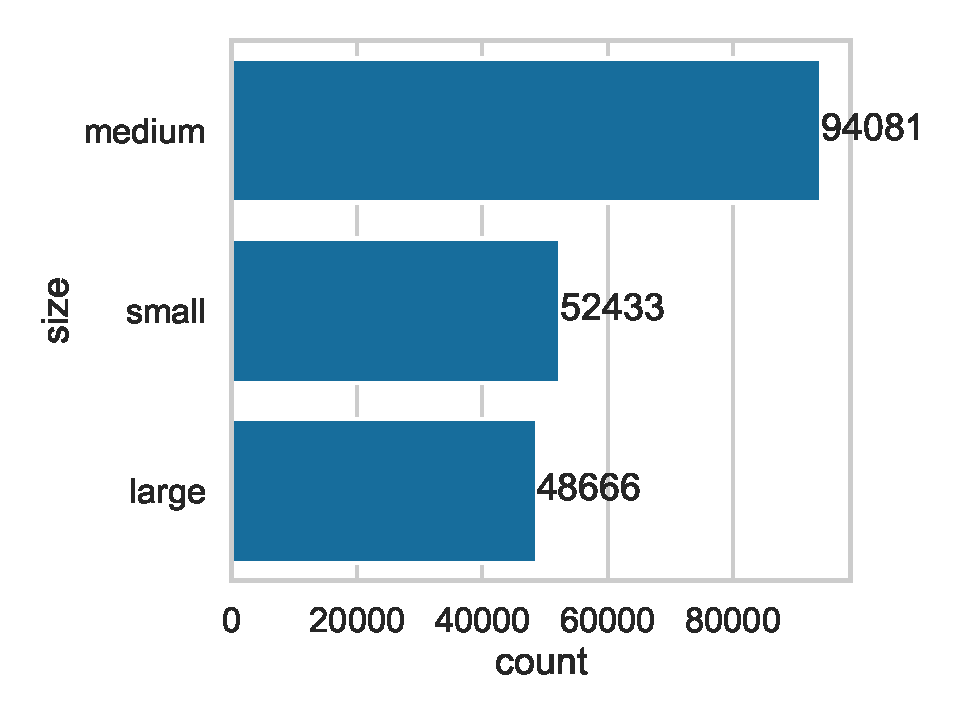
\includegraphics[width=0.5\textwidth]{notebook-size-distribution.pdf}
  \caption{Number of notebooks in the small, medium and large notebook size categories.}
  \label{fig:notebook-size-distribution}
\end{figure}

\begin{figure}
  \centering
  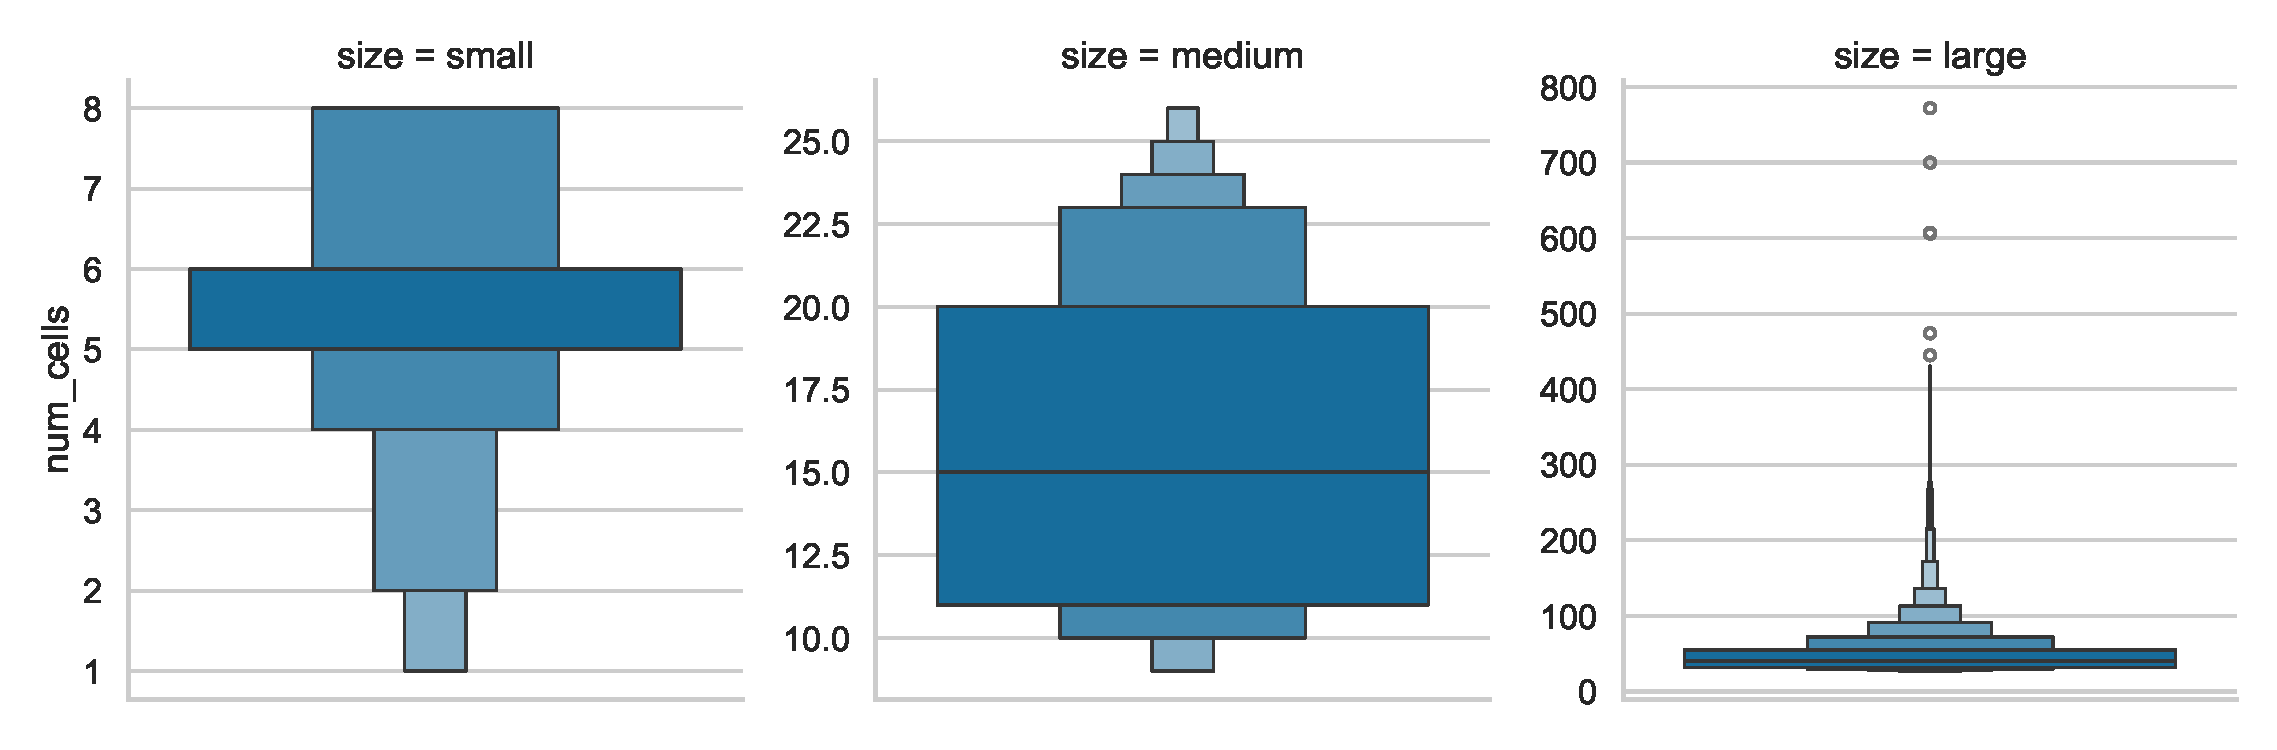
\includegraphics[width=0.75\textwidth]{cell-per-notebook-size-distribution.pdf}
  \caption{Distribution of number of cells in all notebook size categories.}
  \label{fig:cell-per-notebook-size-distribution}
\end{figure}

\begin{figure}
  \centering
  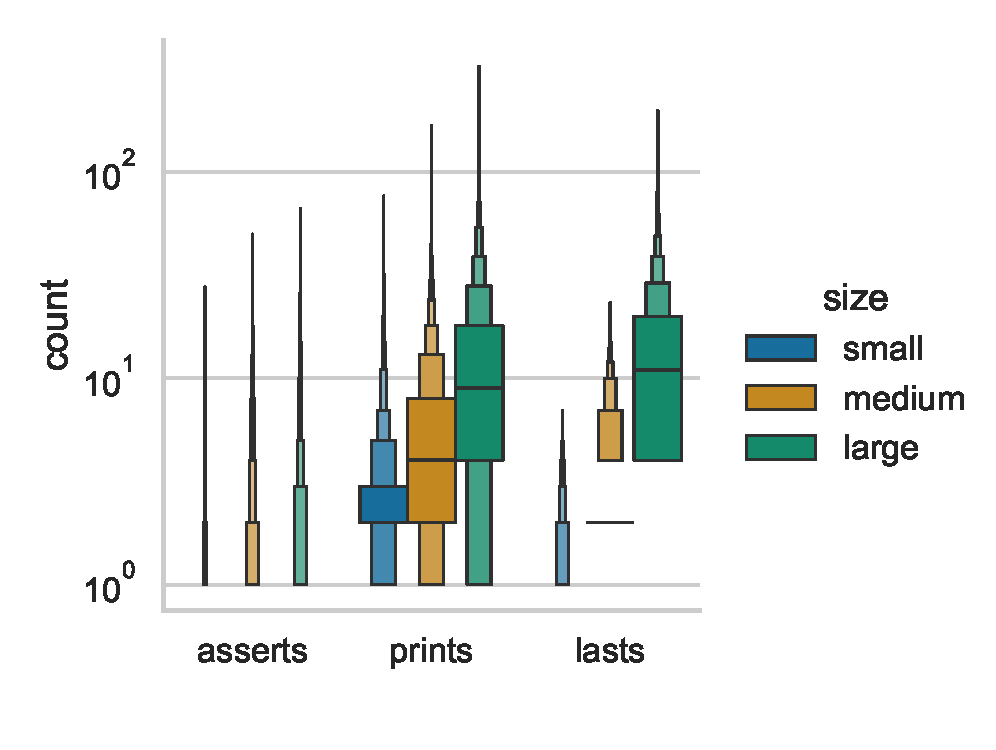
\includegraphics[width=0.5\textwidth]{fms-per-notebook-size-distribution.pdf}
  \caption{Distribution of assertions, prints and last cell statements across all notebook size categories.}
  \label{fig:fms-per-notebook-size-distribution}
\end{figure}

Following is the text from section 4.1 Descriptive Statistics which was added to the manuscript to address this comment.

\begin{quote}
  Figure 4 shows the distribution of the number of code cells for all notebooks analyzed in this study. The distribution is grouped into three categories---namely small, medium and large---based on the first and third quartiles. This is done since the data is large, non-uniform and contains many outliers. Figure 5 further magnifies the distribution of the number of cells within each category. The dataset mostly contains medium size notebooks (9 to 26 code cells), followed by small (1 to 8 code cells) and large (27 to 772 code cells) size notebooks.

  Figure 6 shows the distribution of assertions, prints and last cell statements across the different notebook size categories. A logarithmic scale is used for the count since the data is large and contains outliers. Overall, the visualization suggests an increase in the use of all feedback mechanisms as notebook size grows. Print statements are the most frequently used across all notebook sizes.
\end{quote}

\begin{revcomment}[2.4]
  Additionally, stratifying the dataset based on notebook complexity (e.g., single-cell, small-scale, medium-scale, and large-scale notebooks) and analyzing feedback mechanisms within these clusters would enhance the study's depth.

  For instance:
  \begin{itemize}
    \item Single-cell notebooks might represent quick experiments or incomplete workflows, potentially over-relying on print statements for debugging.
    \item Small- to medium-scale notebooks could exhibit more balanced feedback mechanisms, such as assertions validating intermediate results.
    \item Large-scale notebooks might show structured practices with complete feedback mechanisms aimed at reproducibility and production-readiness.
  \end{itemize}

  By analyzing whether the findings hold consistently across these clusters, the authors could find patterns specific to notebook complexity. This approach would not only validate the robustness of the results but also provide more targeted recommendations for practitioners working with notebooks of varying complexity. Including this stratified analysis would significantly strengthen the study's contributions.
\end{revcomment}

\Us Thank you for your feedback. We explored the idea of using notebook size (number of cells) as a proxy for complexity. However, we found that larger notebooks don't necessarily contain more complex feedback mechanisms, and smaller notebooks can sometimes contain sophisticated feedback constructs. For example, the largest notebook in our dataset contains over 500 simple print statements (see large-notebook.ipynb: \url{https://surfdrive.surf.nl/files/index.php/s/FDQkCFxQNAVZIcq}), while some compact notebooks implemented complex assertion patterns with custom validation logic (see small-notebook.ipynb: \url{https://surfdrive.surf.nl/files/index.php/s/FDQkCFxQNAVZIcq}).

To avoid making assumptions about the relationship between notebook size and feedback mechanism complexity, we opted for stratified random sampling based on TF-IDF values. This approach ensures a diverse population of feedback mechanisms in our analysis, giving appropriate representation to both common patterns and specialized implementations regardless of the notebook size.

Additionally, we have added section 5.6 Complexity of Notebooks that discusses the existing challenges of defining notebook complexity and its potential value to improve the depth of this study as future work. While we agree that analyzing the complexity of notebooks may lead to interesting patterns, it is however difficult to define notebook complexity. We agree that the number of cells (or size) of a notebook is a valid albeit not the only metric that should be considered to define notebook complexity.

Following is the text that was added to section 5.6 Complexity of Notebooks to address this comment.

\begin{quote}
  Analyzing the feedback mechanisms with respect to the complexity of Jupyter notebooks remains a promising direction for future research. We believe that the primary challenge here will be to develop an appropriate definition for notebook complexity.

  To the best of our knowledge, no formal definition or metrics to quantify notebook complexity exist to date. In their research, Grotov et al. (2022) investigated the complexity of Python code written inside Jupyter notebooks using a subset of 15 metrics derived from prior literature. These metrics however were primarily developed for code structured in an object-oriented programming paradigm. Consequently, the applicability of these metrics to code within notebooks is questionable, particularly given that research indicates notebooks frequently diverge from established software engineering best practices (Pimentel et al., 2019).

  It is further unclear how metrics such as the size of the training data, complexity of the learning algorithm, computational costs and CO\(_2\) emissions associated with training can be incorporated into the definition for notebook complexity. Addressing these challenges would facilitate the stratification of our dataset into distinct categories---namely low, medium, and high complexity---which can enhance the depth of this study by enabling a more nuanced analysis of feedback mechanisms within this context.

\end{quote}

\begin{revcomment}[2.5]
  The use of TF-IDF scores to sample feedback mechanisms for case studies prioritizes textual uniqueness. This approach risks overemphasizing rare but trivial feedback, such as simple debugging statements (print("Hello world")), while potentially underrepresenting more common but functionally critical feedback. Incorporating functional complexity or analyzing interdependencies between feedback mechanisms and other cells would improve sampling relevance.
\end{revcomment}

\Us Thank you for your feedback. We have revised section 3.2 Exploratory Case Study Analysis to explicitly mention the bias introduced by using TF-IDF and how subsequently the stratified random sampling is used to mitigate this threat.

Following is the relevant text from the revised version of section 3.2 Exploratory Case Study Analysis which was added to address this comment.

\begin{quote}
  The assertions, print statements and last cell statements are first tokenized---special characters and alphanumeric words shorter than two characters are removed. Two stop words namely ``assert'' and ``print'' are removed since they appear in all assertions and print statements respectively. The term frequency (TF) for the remaining tokens is calculated and then normalized using their inter-document frequency (IDF). This normalization process assigns higher values to tokens that are less frequently encountered, which can lead to overemphasis of candidates that contain rare tokens. Consider for instance, the trivial print statement \texttt{print("hello, world!")}. Since this statement does not commonly appear in the context of machine learning Jupyter notebooks, it will have a high TF-IDF score but adds little substantive value to the analysis.

  To address the potential bias introduced by this method, we employ stratified random sampling to select candidates for the case study analysis. The subgroups are created based on the aggregated TF-IDF values of the tokens in each candidate. The candidates are then divided into quartiles based on the aggregate value. As a result, all candidates characterized by rare tokens are grouped within a single bin. By randomly selecting candidates from each bin, we ensure that the final population reflects a diverse mix of candidates, mitigating the risk of over representing those that are trivial yet rare.
\end{quote}

\begin{revcomment}[2.6]
  Machine learning workflows vary significantly by task (e.g., classification, regression, clustering). Different tasks require different feedback mechanisms—for example, assertions about image dimensions in computer vision or data distribution checks in NLP. Analyzing the dataset by ML task type would provide targeted insights and make the recommendations more actionable for practitioners.
\end{revcomment}

\Us Thank you for your feedback. We have revised section 5.4 Machine Learning Bugs to discuss feedback mechanisms and machine learning workflows.

Following is the relevant text added to section 5.4 Machine Learning Bugs.

\begin{quote}
  This study further reveals several avenues for future research. We primarily focused on identifying feedback mechanisms used when writing ML code in Jupyter notebooks and subsequently exploring a limited subset of them. Further research is required to investigate these feedback mechanisms in greater depth and systematically organize them into a taxonomy grounded in specific ML validation tasks. It is important to recognize that machine learning workflows vary significantly across different tasks---such as classification, regression, and clustering. Each task necessitates distinct feedback mechanisms. For instance, assertions regarding image dimensions are pertinent in computer vision, whereas data distribution checks are critical in natural language processing. By analyzing the dataset according to the specific types of ML tasks, researchers can obtain targeted insights, thereby enhancing the practicality and applicability of recommendations for practitioners.
\end{quote}

\begin{revcomment}[2.7]
  2. Feedback mechanisms and their context

  Jupyter notebooks allow for out-of-order execution, which impacts the effectiveness of feedback mechanisms. A statement such as print(``Accuracy:'', accuracy) is only useful if the cell defining accuracy has been executed first. The paper partially explore how such dependencies affect the functionality of feedback mechanisms, leaving a gap in the analysis.

\end{revcomment}

\Us Thank you for your feedback. We have added section 5.7 Reproducibility of Jupyter Notebooks to improve the discussion on feedback mechanisms and how their functionality is affected during out-of-order execution of cells.

Following is the text that was added to section 5.7 Reproducibility of Jupyter Notebooks.

\begin{quote}
  Code written within Jupyter notebooks can reach a convoluted state since the code cells can be executed in any order. Each time a cell is run, it updates the state of the program within the kernel, leading to the potential for discrepancies if cells defining variables or functions are executed after cells that depend on them. Such out-of-order execution may result in a situation where subsequent cells operate on outdated or undefined values, ultimately complicating the workflow and undermining the reproducibility of ML experiments (Pimentel et al., 2019; Wang et al., 2020b).

  The assertions presented in Section 4.3 can be used to enhance the reproducibility of ML experiments by ensuring that consistent validation checks are applied, irrespective of the execution order of the notebook cells (Wang et al., 2020b). Conversely, implicit feedback constructs like \texttt{print(``Accuracy:'', accuracy)} are only effective if the cell defining \texttt{accuracy} has been executed prior to the print statement. In this paper, we have partially examined how these dependencies influence the functionality of feedback mechanisms, highlighting the complexities involved in maintaining reproducibility in scenarios where cell execution order is not strictly linear. Further investigation in this area could provide important insights into optimizing the use of assertions and other feedback mechanisms in Jupyter notebooks, particularly in the context of diverse ML workflows.
\end{quote}

\begin{revcomment}[2.8]
  The paper treats all print statements and last cell outputs as feedback mechanisms. However, many of these may be incidental, such as debugging statements or placeholders that do not provide actionable feedback. Distinguishing intentional feedback from debugging artifacts would refine the analysis. What about introducing criteria for identifying feedback mechanisms that actively influence decision-making versus those used for temporary debugging?
\end{revcomment}

\Us Thank you for your feedback. As per our original definition of feedback mechanisms from section 1 Introduction, all print statements are considered as feedback mechanisms in this study.

Regardless, we have revised the definition of feedback mechanisms in the introduction, clearly emphasized the difference between implicit and explicit feedback, and clarified how they differ from testing.

Following is the revised text from section 1 Introduction that was added to address this comment.

\begin{quote}
  Within this environment, feedback mechanisms are essential for improving code quality and diagnosing issues. \textbf{Feedback mechanisms are tools or techniques intentionally integrated into the code by the developer to gain insight into the execution of the program}. Importantly, not all forms of feedback quality as feedback mechanisms. For example, a bug in the code may produce feedback indicating an issue, but because the bug was not intentionally inserted, it does not count as a feedback mechanism.

  Notebook users can obtain feedback using implicit or explicit mechanisms. \textbf{Implicit feedback mechanisms require manual validation by the user}. For instance, a common prerequisite for all ML models is that the features in the dataset are all numerical. This can be verified with a print statement in a code cell and manually checking the output. This code statement however, will continue to execute even if the data type of a feature changes in subsequent batches of training data.

  In contrast, \textbf{explicit feedback mechanisms document the expected conditions of the code and halt execution if these conditions are not met}. For instance, the implicit validation method mentioned above can be replaced with an explicit assertion: \texttt{assert all(df[col].dtype in ['int64', 'float64'] for col in df.columns), "Not all columns are of numerical type"}. This assert statement will stop the execution if the condition is not satisfied and provide immediate feedback with a clear message explaining the issue.

  It is important to contextualize feedback mechanisms within the broader framework of software testing. Traditional testing methodologies employ formal tests to explicitly identify discrepancies between expected and actual code functionality. \textbf{While all tests serve as feedback mechanisms, not all feedback mechanisms operate within this formal testing paradigm}. For instance, print statements and outputs from the last statement of code cells offer a more informal approach to gaining insights into the execution status and data flow within a Jupyter notebook. While such implicit feedback types can help practitioners diagnose issues within their code, they necessitate manual validation and interpretation, which can increase the potential for oversight and errors.
\end{quote}

\begin{revcomment}[2.9]
  The authors position assertions as superior to implicit mechanisms like print statements. While this aligns with software engineering principles, no empirical evidence is provided to show that assertions lead to more reliable workflows in practice. For instance, assertions may be less suitable for exploratory phases, where rapid visual feedback is often preferred.
\end{revcomment}

\Us Thank you for your feedback. We acknowledge that the current study does not provide empirical evidence to support the claim that explicit feedback mechanisms are superior to their implicit counterparts. However, the manuscript does support this statement with sufficient theory building found in section 1 Introduction and extensively throughout section 5 Discussion. Regardless, we have revised section 5.2 Automated Data Validation to explicitly state this as future work.

Following is an excerpt from section 5.2 Automated Data Validation added to address this comment.

\begin{quote}
  The results from RQ2 indicate that assertions can be used to automatically validate critical assumptions in ML workflows. Embedding assertions into the code helps ensure that any deviation from expected conditions is promptly flagged. This reduces the reliance on manual verification thus enhancing the robustness and maintainability of ML pipelines. Assertions also serve as an executable form of documentation that captures the assumptions and decisions made during model development. This is particularly important in collaborative environments where multiple practitioners might work on the same project. Assertions ensure that all team members have a clear understanding of the requirements and constraints across the entire ML pipeline, facilitating smoother transitions and handovers. Future work can focus on providing empirical evidence to demonstrate that the integration of assertions significantly improves the reliability of ML workflows in practice.
\end{quote}

\begin{revcomment}[2.10]
  3. Recommendations and practical relevance

  Development phase considerations: feedback needs differ across development stages. For instance, print statements may be more valuable during early exploration, while assertions are more appropriate for production workflows. Recommendations that account for these stages would make the findings more useful.
\end{revcomment}

\Us Thank you for your feedback. We agree with this point of view that as ML pipelines developed inside Jupyter notebooks mature, the implicit feedback mechanisms should be converted to explicit feedback mechanisms as per software engineering best practices. Here is an excerpt from section 1 Introduction of the manuscript that motivates this recommendation.

\begin{quote}
  As machine learning pipelines developed within Jupyter notebooks become business-critical, they are frequently transitioned into automated scripts for production environments (Kery et al., 2018; Rule et al., 2018). In these contexts, it is crucial to shift from implicit feedback mechanisms to explicit ones. This transition reduces the reliance on manual verification, thereby enhancing the robustness and maintainability of ML pipelines.
\end{quote}

We also believe that existing feedback mechanisms in the notebooks (implicit and explicit) can make the transition from notebooks into a production environment smoother. In section 5.1 Documentation and Technical Debt we highlight how artifacts---such as requirements, rationale and design decisions and tests---which are a prerequisite for all operational software systems, can be effectively derived from the feedback mechanisms used inside notebooks. Furthermore, in section 5.2 Automated Data Validation, we propose that assertions can be used to derive the data validation schema for dedicated data validation tools, which are often incorporated into operational ML pipelines.

Following are the relevant excerpts from section 5.1 Documentation and Technical Debt and 5.2 Automated Data Validation respectively that support the above statement.

\begin{quote}
  Jupyter notebooks are primarily used to explore different ideas or approaches [\ldots] In both scenarios, practitioners need to revisit the notebooks to obtain up-to-date and accurate requirements, their rationale and design decisions, and tests---artifacts which are usually missing in the original notebooks (Pimentel et al., 2019; Psallidas et al., 2019; Grotov et al., 2022).

  Our findings indicate that structured information can be effectively derived from the feedback mechanisms available in Jupyter notebooks. The results demonstrate that practitioners utilize assertions, print statements, code cell outputs, and visualizations to inform data preprocessing techniques, detect erroneous assumptions, create new features to enhance model performance, and verify hardware and software dependencies. Moreover, our results from RQ3 reveal [\ldots]
\end{quote}

\begin{quote}
  Results from RQ2 and RQ3 show that assertions, [\ldots] We argue that when integrating dedicated data validation tools into an operational ML pipeline, the existing feedback mechanisms in notebooks can be effectively used to write the data validation schema.
\end{quote}

We sincerely hope that the clarification provided here is sufficient to address this comment.

\begin{revcomment}[2.11]
  4. Presentation

  Dataset characteristics: detailed statistics on the dataset, such as cell distributions or feedback mechanism frequencies, would improve transparency. These insights would help readers assess the scope and generalizability of the findings.
\end{revcomment}

\Us Thank you for your feedback. We have added section 4.1 Descriptive Statistics to the manuscript which provides additional information regarding the distribution of the number of cells per notebook. Since the data is really large and contains many outliers, we categorized the notebooks into small, medium and large based on the number of cells they contain. Additionally, we also added figures~\ref{fig:notebook-size-distribution},~\ref{fig:cell-per-notebook-size-distribution} and~\ref{fig:fms-per-notebook-size-distribution} to the manuscript, that visualize the distribution of the number of cells and feedback mechanisms across the notebook size categories.

Following is the text from section 4.1 Descriptive Statistics which was added to the manuscript to address this comment.

\begin{quote}
  Figure 4 shows the distribution of the number of code cells for all notebooks analyzed in this study. The distribution is grouped into three categories---namely small, medium and large---based on the first and third quartiles. This is done since the data is large, non-uniform and contains many outliers. Figure 5 further magnifies the distribution of the number of cells within each category. The dataset mostly contains medium size notebooks (9 to 26 code cells), followed by small (1 to 8 code cells) and large (27 to 772 code cells) size notebooks.

  Figure 6 shows the distribution of assertions, prints and last cell statements across the different notebook size categories. A logarithmic scale is used for the count since the data is large and contains outliers. Overall, the visualization suggests an increase in the use of all feedback mechanisms as notebook size grows. Print statements are the most frequently used across all notebook sizes.
\end{quote}

\begin{revcomment}[2.12]
  While the authors acknowledge constraints, such as the reliance on public datasets, other limitations could be better discussed. For example, the absence of task-specific analysis or a lack of industrial datasets could affect the applicability of the findings. Addressing these explicitly would strengthen the paper's credibility.
\end{revcomment}

\Us Thank you for your feedback. We have made several revisions to the manuscript to address this comment. We have revised section 3.2 Exploratory Case Study Analysis to explicitly highlight the limitations and threats of our current approach and how we mitigate this threat. All subsections under section 5 Discussion have been updated to state limitations of the current work and potential directions for future work. Two new sections 5.6 Complexity of Notebooks and 5.7 Reproducibility of Notebooks were also added to the Discussion section. Finally, we have also revised section 6 Threats to Validity the address the limitations of the study explicitly.

You may also refer to our response to comments 1.5, 2.4 and 2.7 along with the diff document for additional details.

\begin{revcomment}[2.13]
  Summary of the suggestions

  \begin{itemize}
    \item present detailed statistics on the dataset, such as the distribution of cells per notebook and task annotations.
    \item analyze feedback patterns by ML task type to provide domain-specific insights.
    \item distinguish debugging statements from intentional feedback mechanisms.
    \item provide phase-specific recommendations for exploratory versus production workflows.
    \item better discuss broader limitations, including the dataset's reliance on public repositories and its implications for generalizability.
  \end{itemize}

  Overall, this paper is a well-organized and interesting exploration of feedback mechanisms in ML workflows. Its large-scale dataset and systematic approach provide a solid starting point for understanding feedback practices in Jupyter notebooks. The suggestions outlined in this review are intended as constructive feedback to further refine the study and explore additional dimensions that could enhance its applicability and depth. The paper addresses an important and underexplored area, and it offers important insights that will likely inspire future research in this domain.
\end{revcomment}

\Us Thank you for your valuable feedback and comments.

\newreviewer{3}
\begin{revcomment}[3.1]
  \textbf{Paper Summary}

  This paper researches how machine learning (ML) developers using Jupyter Notebooks implement feedback mechanisms during the ML development process. The authors identify two primary types of feedback: implicit and explicit. The authors indicate that implicit feedback is typically provided through print statements and the output of the last cell in the notebook, while explicit feedback is provided by assert statements. To investigate these mechanisms, the authors analyzed a dataset of 297.8 thousand Jupyter Notebooks. They explain the process of gathering the data, and removing the duplicates. From this dataset, they closely examined 82 assert statements, 44 print statements, and 27 last cell outputs to further understand their purposes. The authors state that their findings reveal that implicit feedback is significantly more commonly used than explicit feedback. Additionally, the paper includes a detailed analysis of the most frequently used methods in assert statements, as well as the most common constructs employed in print statements and last-cell outputs. Finally, the author discusses some of the implications of their findings in regards to their implications with respect to different aspects like documentation and technical debt.

  \textbf{Strengths and Weaknesses}

  \textbf{Strengths:}
  \begin{itemize}
    \item The authors provide a detailed background, explaining several of the concepts introduced in the paper.
    \item The dataset used in the study is available online.
  \end{itemize}

  \textbf{Weaknesses:}
  \begin{itemize}
    \item The authors do not define the term feedback explicitly anywhere in the paper.
    \item Many claims are more general than they should be.
    \item The findings needs to have a deeper implication analysis earlier in the results section rather than later in the discussion.
    \item The reason for some study design decisions are not explained clearly like the limit of the analysis to 200 hours or use of TF-IDF for selection in the case studies section.
    \item The author claim that this is the first study to look into feedback mechanism in ML projects, they need to focus their claim on Juypter notebook rather than wider ML projects.
  \end{itemize}
\end{revcomment}

\Us Thank you for your valuable comments and feedback.

\begin{revcomment}[3.2]
  \textbf{Comments to Authors}

  I find that the paper, as it stands, doesn't read smoothly. The big picture is unclear, and I often find myself wondering, ``So what?'' It feels like the focus was too heavily placed on numbers and detailed nuances, with less attention given to the paper's narrative. For example, the term feedback is never explicitly defined. Additionally, I find that some claims in the paper, such as the one mentioned in the abstract, come across as unsupported. In addition, given that the paper's first keyword is SE4AI, I expected a stronger software engineering perspective on the process, like how the findings align or differ from best practices, what are some alternative practices not found in the results, or how effective these are mechanism and what are their limitation. Instead, the paper focuses primarily on numerical results and data analysis, with the discussion section addressing some of those aspects but not effectively.
\end{revcomment}

\Us Thank you for your feedback. We have done our best to address your comments below. We hope that our efforts satisfy your expectations.

\begin{revcomment}[3.3]
  \textbf{Main Questions}

  The following are the major concerns I have about the paper. I think the authors need to address these for the paper to be in good shape for acceptance.

  \begin{itemize}
    \item What exactly do the authors mean by feedback in the ML development process? How does it differ from testing or validation? Although the authors seem to adopt an ``implicit'' understanding of the term, I find this lack of clarity problematic. For instance, they observe ``the limited use of assertions, with only 8.5\% of the notebooks analyzed incorporating them, suggesting a significant gap in current testing practices within the ML community.'' So, it seems they consider it from a testing perspective.
  \end{itemize}
\end{revcomment}

\Us Thank you for your feedback. We have revised section 1 Introduction to clearly define feedback mechanisms, emphasize the difference between implicit and explicit feedback, and clarify how they differ from formal testing.

Following is the text that was added to section 1 Introduction to address this comment. We sincerely hope that the new text is sufficient to address the concern raised in this comment.

\begin{quote}
  Within this environment, feedback mechanisms are essential for improving code quality and diagnosing issues. Feedback mechanisms are tools or techniques intentionally integrated into the code by the developer to gain insight into the execution of the program. Importantly, not all forms of feedback quality as feedback mechanisms. For example, a bug in the code may produce feedback indicating an issue, but because the bug was not intentionally inserted, it does not count as a feedback mechanism.

  Notebook users can obtain feedback using implicit or explicit mechanisms. Implicit feedback mechanisms require manual validation by the user. For instance, a common prerequisite for all ML models is that the features in the dataset are all numerical. This can be verified with a print statement in a code cell and manually checking the output. This code statement however, will continue to execute even if the data type of a feature changes in subsequent batches of training data.

  In contrast, explicit feedback mechanisms document the expected conditions of the code and halt execution if these conditions are not met. For instance, the implicit validation method mentioned above can be replaced with an explicit assertion: \texttt{assert all(df[col].dtype in ['int64', 'float64'] for col in df.columns), "Not all columns are of numerical type"}. This assert statement will stop the execution if the condition is not satisfied and provide immediate feedback with a clear message explaining the issue.

  It is important to contextualize feedback mechanisms within the broader framework of software testing. Traditional testing methodologies employ formal tests to explicitly identify discrepancies between expected and actual code functionality. While all tests serve as feedback mechanisms, not all feedback mechanisms operate within this formal testing paradigm. For instance, print statements and outputs from the last statement of code cells offer a more informal approach to gaining insights into the execution status and data flow within a Jupyter notebook. While such implicit feedback types can help practitioners diagnose issues within their code, they necessitate manual validation and interpretation, which can increase the potential for oversight and errors.
\end{quote}

\begin{revcomment}[3.4]
  \begin{itemize}
    \item For the print statements and last cell outputs, how do the authors determine that their purpose is related to feedback rather than other purposes, or do they consider all print statements as feedback mechanisms?
  \end{itemize}
\end{revcomment}

\Us Thank you for your feedback. Yes, as per the revised definition of feedback mechanisms in section 1 Introduction, all print statements are considered feedback mechanisms.

You may also see our response to comment 3.3 above for further details.

\begin{revcomment}[3.5]
  \begin{itemize}
    \item The authors need to justify their study choices more explicitly. For instance:
    \item Why limit the analysis to Jupyter Notebooks? While they mention their ubiquity, their claim seems to broadly target ML projects. If their scope is strictly Jupyter Notebooks, they need to focus their claims on those rather than the wider ML community.
  \end{itemize}
\end{revcomment}

\Us Thank you for your feedback.

After careful consideration, we believe that although the analysis in this study was conducted using Jupyter notebooks, the findings are applicable to other computational notebook technologies which follow the same REPL based paradigm of software development. We have therefore revised section 6 Threats to Validity (External Validity) to clarify the scope of this study.

Following is the revised text from section 6 Threats to Validity (External Validity).

\begin{quote}
  Our analysis is based on ML notebooks that are publicly available on platforms such as GitHub and Kaggle. As a result, the findings may not be generalizable to Python notebooks that do not center around ML applications. Furthermore, the applicability of the results is limited when it comes to notebooks authored in other statistical programming languages, such as R or Julia.

  The analysis in this study is conducted only using Jupyter notebooks. However, the underlying workflow of users across all notebook environments is identical---that is, users execute chunks of code using a REPL mechanism. As such, the findings of this study may be generalizable to other notebook technologies.
\end{quote}

\begin{revcomment}[3.6]
  \begin{itemize}
    \item Why include only notebooks using certain libraries? The authors reference another study, but it's unclear what that study found and how it informed their decision. Adding more detail here would strengthen their argument. They do explain this decision's implications in the threats to validity but it needs to be  explained earlier in the data-gathering part.
  \end{itemize}
\end{revcomment}

\Us Thank you for your feedback. We have revised section 3.1.1 Collection of ML Jupyter Notebooks in the manuscript to clarify the selection criteria using certain Python packages.

Following is the text that was added to section 3.1.1 Collection of ML Jupyter Notebooks to address this comment.

\begin{quote}
  This study focuses on analyzing Python code in Jupyter notebooks with valid JSON structures containing at least one code cell. To concentrate specifically on machine learning projects, we only included notebooks that import at least one major ML library: Scikit Learn (Pedregora et al., 2011), PyTorch (Paszke et al., 2017), TensorFlow (Abadi et al., 2015), or Keras (Chollet et al., 2015). While this approach may exclude some ML projects using alternative libraries, research by Psallidas et al. (2019) examining six million GitHub Jupyter notebooks confirms that most ML-oriented notebooks utilize these frameworks. Despite their widespread usage, we deliberately excluded Pandas, NumPy, and SciPy from our selection criteria as these libraries serve numerous purposes beyond machine learning and are not specifically designed for model training. After applying these filters, we excluded 107 thousand notebooks, resulting in a final dataset of 190.8 thousand notebooks for analysis.
\end{quote}

\begin{revcomment}[3.7]
  I find significant issues with the case studies section. First, it does not include sufficient detail to qualify as a true case study; instead, it seems to me that it is an exploratory analysis of the purpose of some instances of the feedback mechanisms. Additionally, the author needs to better explain the rationale for using TF-IDF for selection, and the decision to limit the analysis to 200 hours seems arbitrary.
\end{revcomment}

\Us Thank you for your feedback. We made several adjustments to the manuscript to address this comment. We renamed the title of section 3.2 Case Studies to \emph{Exploratory Case Study Analysis} to be verbose about the methodology. We added more details regarding the \emph{site} and the \emph{selection criteria} of the study. Furthermore, details regarding the sampling technique using TF-IDF, the bias introduced, and our mitigation strategy using stratified random sampling has also been added.

Finally, to validate the taxonomy of feedback mechanisms, the second author independently annotated all candidates using the codes that were generated during the first round of annotations. We have reported the inter-rater agreement which was calculated using the \emph{Cohen's Kappa} metric in the manuscript.

Following is the revised text from section 3.2 Exploratory Case Study Analysis where we addressed the concerns raised in this comment.

\begin{quote}
  For RQ2 and RQ3, we allocated a fixed time resource of 200 hours to conduct the exploratory case study analysis of all candidate assertions, print statements and last cell statements. We specified Jupyter notebooks written in the Python programming language as the \emph{site} for the study. Given the exploratory nature of this study, we emphasized capturing a diverse range of candidates by apply text processing and sampling techniques as described below.

  The assertions, print statements and last cell statements are first tokenized---special characters and alphanumeric words shorter than two characters are removed. Two stop words namely ``assert'' and ``print'' are removed since they appear in all assertions and print statements respectively. The term frequency (TF) for the remaining tokens is calculated and then normalized using their inter-document frequency (IDF). This technique allows us to surface both frequently occurring feedback mechanisms and those that are rarer in the dataset.

  This normalization using IDF assigns higher values to tokens that are less frequently encountered, which can lead to overemphasis of candidates that contain rare tokens. Consider for instance, the trivial print statement \texttt{print("hello, world!")}. Since this statement does not commonly appear in the context of machine learning Jupyter notebooks, it will have a high TF-IDF score but adds little substantive value to the analysis.

  To address the potential bias introduced by this method, we employ stratified random sampling to select candidates for the case study analysis. The subgroups are created based on the aggregated TF-IDF values of the tokens in each candidate. The candidates are then divided into quartiles based on the aggregate value. As a result, all candidates characterized by rare tokens are grouped within a single bin. By randomly selecting candidates from each bin, we ensure that the final population reflects a diverse mix of candidates, mitigating the risk of overrepresenting those that are trivial yet rare.

  During each case study, the first author categorized each candidate using \emph{inductive coding}. The first author analyzed the Python code of the candidate to understand its purpose. Additionally, the entire code cell, the previous cell, next cell and the notebook's purpose was analyzed to bring in rich context. For case studies where the first author was unable to determine the purpose of the candidate, it was additionally analyzed by the second and third authors. Finally, the entire research team held regular meetings throughout this iterative process to ensure consistency in the categorization of the feedback mechanisms.

  A taxonomy of feedback mechanisms observed in ML Jupyter notebooks was created using the categories generated during the exploratory case study analysis. To validate the taxonomy developed by the first author, the second author independently annotated the candidates using the categories developed by the first author. The inter-rater agreement was calculated using the \emph{Cohen's Kappa} method and a score 0.8 was obtained which is regarded as highly agreeable.
\end{quote}

We have also revised section 6 Threats to Validity (Internal Validity) to discuss the pros and cons of using a fixed time resource. While we agree that the use of a fixed time resource has limitations, other stopping criteria, such as those based on theoretical saturation, are also subject to bias from the annotator. In contrast to other methods, a fixed time resource reflects the practical resource constraints that researchers face in the real world. Furthermore, our goal for the study was not to create an extensive taxonomy of feedback mechanisms but to explore if this direction of research warrants future work, and the use of a time budget for the analysis also supports this goal. 

Following is the text that was added to section 6 Threats to Validity (Internal Validity) to address this comment.

\begin{quote}
  We enforced a time resource limit of 200 hours for conducting the case studies in RQ2 and RQ3, potentially constraining the depth and breadth of our investigation. Although alternative stopping rules such as theoretical saturation are common, they are inherently subjective and can vary based on the judgement of a researcher. In contrast, a time-bound method ensures transparency and reflects the practical resource constraints in real-world research. Additionally, the stratified random sampling [\ldots]
\end{quote}

We sincerely hope that the revisions are sufficient to address the concerns raised by this comment.

\begin{revcomment}[3.8]
  Some of the findings seem fairly intuitive such as ``Finding 1.3 Print statements are commonly used to display various performance metrics of ML models'' and Finding 1.4 ``Libraries and functions for data visualization, data exploration and machine learning are most common in last cell statement''. These findings align with standard practices in ML. I think the authors need to provide a deeper analysis of their implications. The author may consider examining when does these feedback mechanism happen in the development lifecycle, how effective they are, or what does these finding implies in regards to best practices in respect to software engineering for ML. I do see that they reference the findings in general in the discussion section, touching on their implications. Still, it is better to add specific implications for each finding in the results section.
\end{revcomment}

\Us Thank you for your feedback. While we agree that some observations may seem intuitive and obvious, we still report all observations of the study for completeness. We have made significant revisions to the discussion section to improve the analysis and provide deeper implications. To summarize, we revised all subsections under section 5 Discussion to include additional details such as limitations of the current work, potential directions for future work and implications for notebook users and developers. We also added two new subsections under section 5 Discussion to further enhance the implications of the study. We hope that these revisions meet your expectations.

You may also refer to our response for comments 2.9, 2.7, 2.6, 2.4 and 1.2 and the diff document for additional details.

\begin{revcomment}[3.9]
  The authors claim that there has been no prior work investigating feedback in ML projects. However, from a testing perspective, there has been relevant prior research, which the authors may have overlooked. It may be the first study to investigate them in Jupyter Notebook, though, so it is better to be specific. See for example Moses Openja, Foutse Khomh, Armstrong Foundjem, Zhen Ming (Jack) Jiang, Mouna Abidi, and Ahmed E. Hassan. 2024. An empirical study of testing machine learning in the wild. ACM Trans. Softw. Eng. Methodol.
\end{revcomment}

\Us Thank you for your feedback. We have revised section 7.3 ML Testing under related work to acknowledge the overlap with existing research efforts in ML testing.

Following is the text that was added to section 7.3 ML Testing to address this comment.

\begin{quote}
  Despite these advancements, there is a notable gap in practical, day-to-day testing practices within ML development environments. To the best of our knowledge, Openja et al. (2024) is the only study that empirically investigates the test code utilized within 11 ML projects spanning four different application domains. Our study builds upon the findings of Openja at al. (2024) by further analyzing the feedback mechanisms within Jupyter notebooks. We highlight how assertions and print statements are employed to validate data and model performance, and propose strategies for integrating these practices more effectively into the ML development lifecycle.
\end{quote}

\begin{revcomment}[3.10]
  \textbf{Questions related to the Results section:}

  \begin{itemize}
    \item The authors mention grouping candidates based on ``their similarity to each other.'' How is similarity defined?
    \item The case study analysis process needs more detail. The authors note that the first author conducted the analysis, with additional analysis performed by the second and third authors when the author couldn't figure out the purpose of the feedback mechanism. How much of the data was analyzed solely by the first author versus collaboratively? Did the authors analyze the inter-rater agreement?
    \item Add a clearer explanation of the findings' implications.
  \end{itemize}
\end{revcomment}

\Us Thank you for your feedback. We have made several revisions to section 3.2 Exploratory Case Study Analysis to address this comment. In summary, we added more details regarding the exploratory case study analysis and how the first round of analysis was conducted by the first author to create the taxonomy of feedback mechanisms. To validate the codes of the taxonomy, the second author independently did a second round of annotations. We calculated the inter-rater agreement using the \emph{Cohen's Kappa} metric (we report a score of 0.8, highly agreeable).

You may also refer to our response for comment 3.7 and the diff document for additional details.

\begin{revcomment}[3.11]
  \textbf{Questions related to the Discussion section:}

  Many of the implications stated in the discussion section are not directly backed up by the findings of the study or grounded in the existing literature. For example:

  \textbf{Documentation and Technical Debt:}

  \begin{itemize}
    \item The author's argument in this section is somewhat vague. They state that their study ``provides a valuable resource for ongoing efforts to automatically generate documentation from code written in Jupyter notebooks.'' Make it clearer what these efforts are and how exactly their study contributes to them.
  \end{itemize}
\end{revcomment}

\Us Thank you for your feedback. We have revised section 5.1 Documentation and Technical Debt to address this comment. Following is an excerpt from the revised section 5.1 Documentation and Technical Debt relevant for this comment.

\begin{quote}
  We recommend that ML practitioners document insights derived from implicit feedback mechanisms, especially for visualizations. Visual cues and trends in visualizations are open to interpretation, meaning that different practitioners may interpret the same plot differently (Heer et al., 2010). By documenting these visual insights, practitioners can ensure that the knowledge encapsulated in the visualizations, along with its interpretation and the subsequent decisions made, is preserved and consistently applied throughout the ML lifecycle. Writing documentation from implicit feedback mechanisms and keeping the documentation up-to-date requires significant manual effort. Therein also lies an opportunity for notebook designers and developers to incorporate automated techniques for generating such documentation. We hope that the dataset contributed by this study provides a valuable resource to develop and evaluate such automated tools.
\end{quote}

\begin{revcomment}[3.12]
  \textbf{Automated Data Validation:}

  \begin{itemize}
    \item The authors mention that ``the results from RQ2 indicate that assertions can be used to automatically validate critical assumptions in ML workflows.'' How do the results support this? Additionally, the authors suggest that these results show a ``missed opportunity'' in data validation tasks. What opportunities are they referring to? The authors need to clarify and justify their claims more.
  \end{itemize}
\end{revcomment}

\Us Thank you for your feedback. We have revised section 5.2 Automated Data Validation by making the language clearer to address this comment. Here are the relevant excerpts from the revised section.

\begin{quote}
  The results from RQ2 indicate that assertions can be used to automatically validate critical assumptions in ML workflows. Embedding assertions into the code helps ensure that any deviation from the expected shape of the training data, presence of missing data, and absence of critical resources is promptly flagged. This reduces the reliance on manual verification thus enhancing the robustness and maintainability of ML pipelines.

  Assertions also serve as an executable form of documentation [\ldots]

  Results from RQ2 and RQ3 show that assertions, print statements and last cell statements are predominantly used in the upstream, data-intensive stages of the MLDL. For instance, this study identifies several assertions that perform data validation checks to ensure data meets specific criteria or constraints. Similarly, we find assertions, print statements, and last cell statements that conduct type, shape, and distribution checks to safeguard against data inconsistencies. Based on these results, we argue that when integrating dedicated data validation tools into an operational ML pipeline, the existing feedback mechanisms in notebooks can be effectively used to write the data validation schema.
\end{quote}

\begin{revcomment}[3.13]
  \textbf{Machine Learning Bugs:}

  \begin{itemize}
    \item The discussion on ML bugs is unclear. What is the authors' main point here?
  \end{itemize}
\end{revcomment}

\Us Thank you for your feedback. We have revised Section 5.4 Machine Learning Bugs to address the concern raised by this comment. The primary intent of the section is to highlight how implicit and explicit feedback mechanisms identified in this paper can be connected to existing literature on ML faults and bugs. We additionally revised the section to also highlight future research opportunities.

Following is the revised text from Section 5.4 Machine Learning Bugs

\begin{quote}
  The findings of this study align with prior research on real-world defects in ML systems. Humbatova et al. (2020) propose a taxonomy of faults in DL systems, while Morovati et al. (2023) curate \emph{Defects4ML}, a dataset consisting of ML bugs. Both studies identify defects arising from the use of incorrect data types and shapes, deprecated APIs, and missing GPU resources. Our study identifies several explicit assertions that can catch such data errors. Additionally, we find several implicit checks performed using print and last cell statements to verify the presence of compute resources and libraries, monitor model training, and check the architecture of neural networks. Future work should focus on mapping the feedback mechanisms in Jupyter notebooks to the ML defects identified by Humbatova et al. (2020) and Motovati et al. (2023) which can aid practitioners in debugging or preventing faults using the appropriate feedback technique.

  This study further reveals several avenues for future research. We primarily focused on identifying feedback mechanisms used when writing ML code in Jupyter notebooks and subsequently exploring a limited subset of them. Further research is required to investigate these feedback mechanisms in greater depth and systematically organize them into a taxonomy grounded in specific ML validation tasks. It is important to recognize that machine learning workflows vary significantly across different tasks---such as classification, regression, and clustering. Each task necessitates distinct feedback mechanisms. For instance, assertions regarding image dimensions are pertinent in computer vision, whereas data distribution checks are critical in natural language processing. By analyzing the dataset according to the specific types of ML tasks, researchers can obtain targeted insights, thereby enhancing the practicality and applicability of recommendations for practitioners.

\end{quote}

\end{document}
